\documentclass[french]{article}
\usepackage[utf8]{inputenc}
\usepackage[T1]{fontenc}
\usepackage{lmodern}
\usepackage[a4paper]{geometry}
\usepackage{babel}
\usepackage{graphicx}
\usepackage[colorlinks=true,linkcolor=black,urlcolor=black]{hyperref}

\author{Anthony \textsc{Pena} \and Jérémy \textsc{Bardon}}
\title{\textsc{Scala Basic Editor}\\\normalsize{Projet de Génie Logiciel}\\\hfill{}\\\normalsize{\url{https://github.com/masterALMA2016/scalaBasicEditor}}}
\date{}

\begin{document}
\maketitle

\vspace{3cm}

\renewcommand\contentsname{Sommaire}
\tableofcontents


\newpage

\section{Introduction}

Durant ce projet nous avons mis en place une structure permettant de réaliser un éditeur de texte. Celle-ci a été définie à l'aide de l'outil Papyrus\footnote{Un plugin pour Eclipse, plus d'information ici : \url{http://www.eclipse.org/papyrus/}} et ensuite implémenté en Scala\footnote{Langage de programmation fonctionnel, exécuté sur JVM, plus d'information ici : \url{http://scala.com/fr/}}. Les classes et leurs méthodes ont été testées via des tests unitaires JUnit afin de valider leurs fonctionnements et limiter les bugs.

\section{La structure générale}

\subsection{Editeur}\label{ssec:éditeur}
% conteneur des éléments d'un éditeur
La classe éditeur est une classe assez basique, elle est utilisée pour contenir les différents éléments liés à un éditeur selon les spécifications qui ont été définies. Elle contient principalement deux \texttt{Buffer} (voir \ref{ssec:buffers}) -- un pour la zone de texte et un pour le presse-papier --, un \texttt{Curseur} (voir \ref{ssec:curseur}) et une \texttt{Macro} (voir \ref{sec:macros}).

\subsection{Les buffers}\label{ssec:buffers}
% Une classe, 2 instances : zone de texte + clipboard
% <Figure> des 2 instances ???
% zone de texte et clipboard chacun rien de spé
La classe \texttt{Buffer} est une classe générique de gestion d'un buffer de texte avec les fonctionnalités classiques comme l'ajout de texte -- à la fin ou à une position donnée -- le remplacement d'une portion de texte, la suppression, etc. Dans cette implémentation d'éditeur, le \texttt{Buffer} est utilisé sous la forme de 2 instances : une pour la \og{}\nameref{ssec:zone-texte}\fg{} et une pour le \og{}\nameref{ssec:presse-papier}\fg{}. Les deux éléments ayant des caractéristiques proches (stockage du texte et manipulation de base), il était plus simple de créer une seule classe pour les deux.

\begin{figure}[h!]
	\centering
	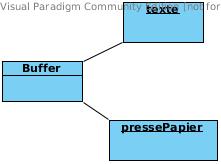
\includegraphics{buffer-texte-clipboard.png}
	\caption{Diagramme d'objet des deux instances de Buffer}
\end{figure}

\subsubsection{Zone de texte}\label{ssec:zone-texte}

La zone de texte est la partie où sera stocké le texte saisie par l'utilisateur. Si on avait développé une interface graphique, cette objet deviendrait une copie côté moteur du contenu affiché à l'utilisateur.

\subsubsection{Presse-papier}\label{ssec:presse-papier}

Le presse-papier est un buffer dans lequel est stocké temporairement le contenu copié par l'utilisateur. Ici nous avons choisi de créer notre propre presse-papier pour simplifier l'implémentation. Si nous avions réalisé complètement l'éditeur nous aurions utilisé à la place l'interface système et son presse-papier afin qu'il soit commun à tous les logiciels.

\subsection{Le curseur}\label{ssec:curseur}
% 2 positions : début + fin
% 		début & fin = -1 => curseur
%		début < fin & fin <> -1 => sélection
% Pour sélectionner : on place le curseur puis on glisse pour définir l'emplacement du curseur de fin, donc on set début puis fin.
Un \texttt{Curseur} est utilisé pour marquer la position à partir de laquelle le texte saisi doit être ajouté. Le \texttt{Curseur} peut aussi servir à définir une sélection. En interne, le \texttt{Curseur} possède deux positions -- \texttt{début} et \texttt{fin} -- lorsqu'on est en \og{}mode saisie\fg{} (pas de sélection), \texttt{fin} est passé à -1 mais dans le cas où une sélection est faite, on assigne une valeur à \texttt{fin}.

Nous avons choisi d'implémenter la sélection comme une action en deux étapes : la première où on place le curseur à une extrémité de la sélection voulue, et la seconde qui consiste à glisser le curseur vers l'autre extrémité de la sélection. Dans le cas où on fait une sélection \og{}négative\fg{} (la seconde extrémité est à gauche du curseur), la sélection est valide et les positions sont inversées.

\section{Les fonctionnalités}\label{sec:fonctionnalités}
% pattern Command
% <Figure> : Editeur, Action, une ou deux actions, Invocateur
% Correspondance avec le nommage du pattern
% Explication choix pattern : beaucoup de fonctionnalité, meilleure évolutivité, séparation "comportement"/"données"
Pour l'implémentation des différentes fonctionnalités nous avons choisi d'utiliser le \texttt{Pattern Commande}\footnote{Une définition complète est disponible à cette adresse : \url{https://fr.wikipedia.org/wiki/Commande_(patron_de_conception)}}. Il nous a permis de séparer données et comportements, ce qui était nécessaire au vu du nombre de fonctionnalités, afin d'éviter d'avoir une classe "dieu" qui ferait tout ou presque. Ce découpage permet aussi une plus grande évolutivité puisqu'une fonctionnalité est contenue dans une classe elle devient par nature facilement extensible pour améliorer son comportement ou en ajouter de nouveaux. Cela donne aussi la possibilité d'effectuer, de manière isolée, des tests sur les différentes fonctionnalités.

Le pattern commande comprend 4 éléments :
\begin{itemize}
	\item \textbf{Commande} est une interface que doivent implémenter les classes de commande.
	\item \textbf{Commande réelle} est un ensemble de classes qui implémente la classe Commande.
	\item \textbf{Invocateur} est la classe sur laquelle on va appeler toutes les commandes comme de simples méthodes. En interne, ce seront les commandes réelles qui seront appelées.
	\item \textbf{Récepteur} est la classe sur laquelle va être appliqué les commandes.
\end{itemize}

\begin{figure}[h!]
	\centering
	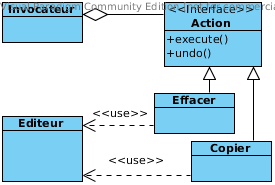
\includegraphics{command-pattern.png}
	\caption{Diagramme de classe des fonctionnalités}
\end{figure}

Dans notre implémentation nous avons utilisé un vocabulaire plus spécifique au projet. Nous avons remplacé commande par \texttt{Action}, les commandes réelles sont les classes \texttt{Copier}, \texttt{Coller}, \texttt{Effacer}, \texttt{Selectionner}, \texttt{Inserer}, \texttt{Deplacer}, \texttt{Remplacer} et \texttt{DeplacerCurseur}, et pour finir le récepteur est la classe \texttt{Editeur}.

\section{Les Macros}\label{sec:macros}
% Pattern Composite
% <Figure> : Macro + Action + autre classe d'action
% une macro est une action, mais composée d'autre actions (et potentiellement d'une autre macro)
% Explication : ne dépend de rien d'autre que de Action => rien à retoucher pour que de nouvelles actions soient ajoutable à une macro

Pour les macros nous avons choisi d'utiliser le Pattern Composite\footnote{Une définition complète est disponible à cette adresse : \url{https://en.wikipedia.org/wiki/Composite_pattern}}, qui est approprié du fait qu'une macro n'est qu'une action composée d'une succession d'actions.

Dans l'implémentation actuelle, le système ne prend qu'une macro en compte, ce qui est suffisant pour tester le fonctionnement des macros, mais on pourrait envisager de permettre l'enregistrement de plusieurs macros. On pourrait aussi donner la possibilité de composer les macros entre-elles, une macro étant défini comme une action à travers le Pattern Composite, cela ne pose aucun problème.

\begin{figure}[h!]
	\centering
	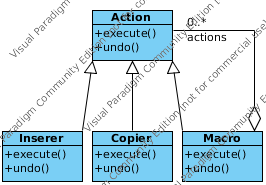
\includegraphics{composite-pattern.png}
	\caption{Diagramme de classe des macros}
\end{figure}


En utilisant ce pattern, on ouvre la possibilité d'étendre la liste des actions possibles sans avoir à modifier la classe \texttt{Macro} du fait qu'une macro est composée d'une série d'action, sans connaitre l'implémentation de chaque action. Il suffit donc que chaque nouvelle action hérite de la classe \texttt{Action} ou d'une de ses sous-classes (c'est le cas de \texttt{Coller} qui hérite de \texttt{Insérer}, la logique étant différente mais la mécanique identique). 


\section{Évolutions}

\subsection{Interface}

Pour aller plus loin dans ce projet, il pourrait être intéressant de créer une interface d'édition. Actuellement seul des tests vérifient que les différents éléments sont fonctionnels mais une interface en ligne de commande -- via ncurses par exemple -- ou graphique permettrait de vérifier que l'implémentation actuelle est fonctionnelle et le projet deviendrait alors utilisable.

\subsection{Nouvelles fonctionnalités}

Il pourrait être intéressant d'étendre les possibilités de l'éditeur. Par exemple en ajoutant la possibilité de sauvegarder plusieurs macros et en permettant de leurs assigner des raccourcis clavier. On pourrait aussi ajouter un fichier de configuration contenant des snippets\footnote{\url{https://en.wikipedia.org/wiki/Snippet_(programming)}} de code. 

\section{Conclusion}
% Structure testé donc normalement fonctionnelle, modulo des erreurs à la mise en application
% Note : Usage Scala = code réduit (+ découverte du langage)
Tout au long de ce projet nous avons pu mettre en pratique les compétences acquises au cours du module de Génie Logiciel et ainsi mettre en application une partie des éléments théoriques comme les Design Pattern dans un projet concret. 

Ce projet nous a aussi permis de découvrir un nouveau langage de programmation et d'utiliser un maximum ces capacités pour mettre en oeuvre notre projet. Le langage Scala permet de produire des binaires portables compatibles avec la JVM, tout en réduisant considérablement la longueur du code, ce qui augmente sa clareté. Nous avons aussi mis en application le module de Tests et Vérifications à travers un certain nombre de tests unitaires, qui nous ont permis de vérifier le bon fonctionnement de nos classes.

%\section{Annexes}

% diagrammes complets

\end{document}